\subsection{Metriche}
Alcune metriche verranno calcolate successivamente con l'avanzare del progetto.\\

I dati fanno riferimento a:
\begin{itemize}
	\item \textbf{A:} Fase di Analisi;
	\item \textbf{PA:} Fase di Progettazione Architetturale;
	\item \textbf{PD} Fase di Progettazione di Dettaglio e codifica (da aggiungere con l'avanzare del progetto);
	\item \textbf{VC: } Fase di Validazione e Collaudo (da aggiungere con l'avanzare del progetto).
\end{itemize}

\subsection{Esiti delle verifiche dell'indice di Gulpease}
Di seguito è riportato il grafico dell'indice di Gulpease calcolato sui vari documenti, il cui valore è definito accettabile e ottimale come descritto nella sezione §2.2.1.1.\\
I dati fanno riferimento a:
\begin{itemize}
	\item \textbf{RR:} Revisione dei Requisiti;
	\item \textbf{RP:} Revisione di Progettazione;
	\item \textbf{RQ:} Revisione di Qualifica (da aggiungere con l'avanzare del progetto);
	\item \textbf{RA:} Revisione di Accettazione (da aggiungere con l'avanzare del progetto).
\end{itemize} 

\subsubsection{Grafico complessivo}

\begin{figure}[H]
\centering
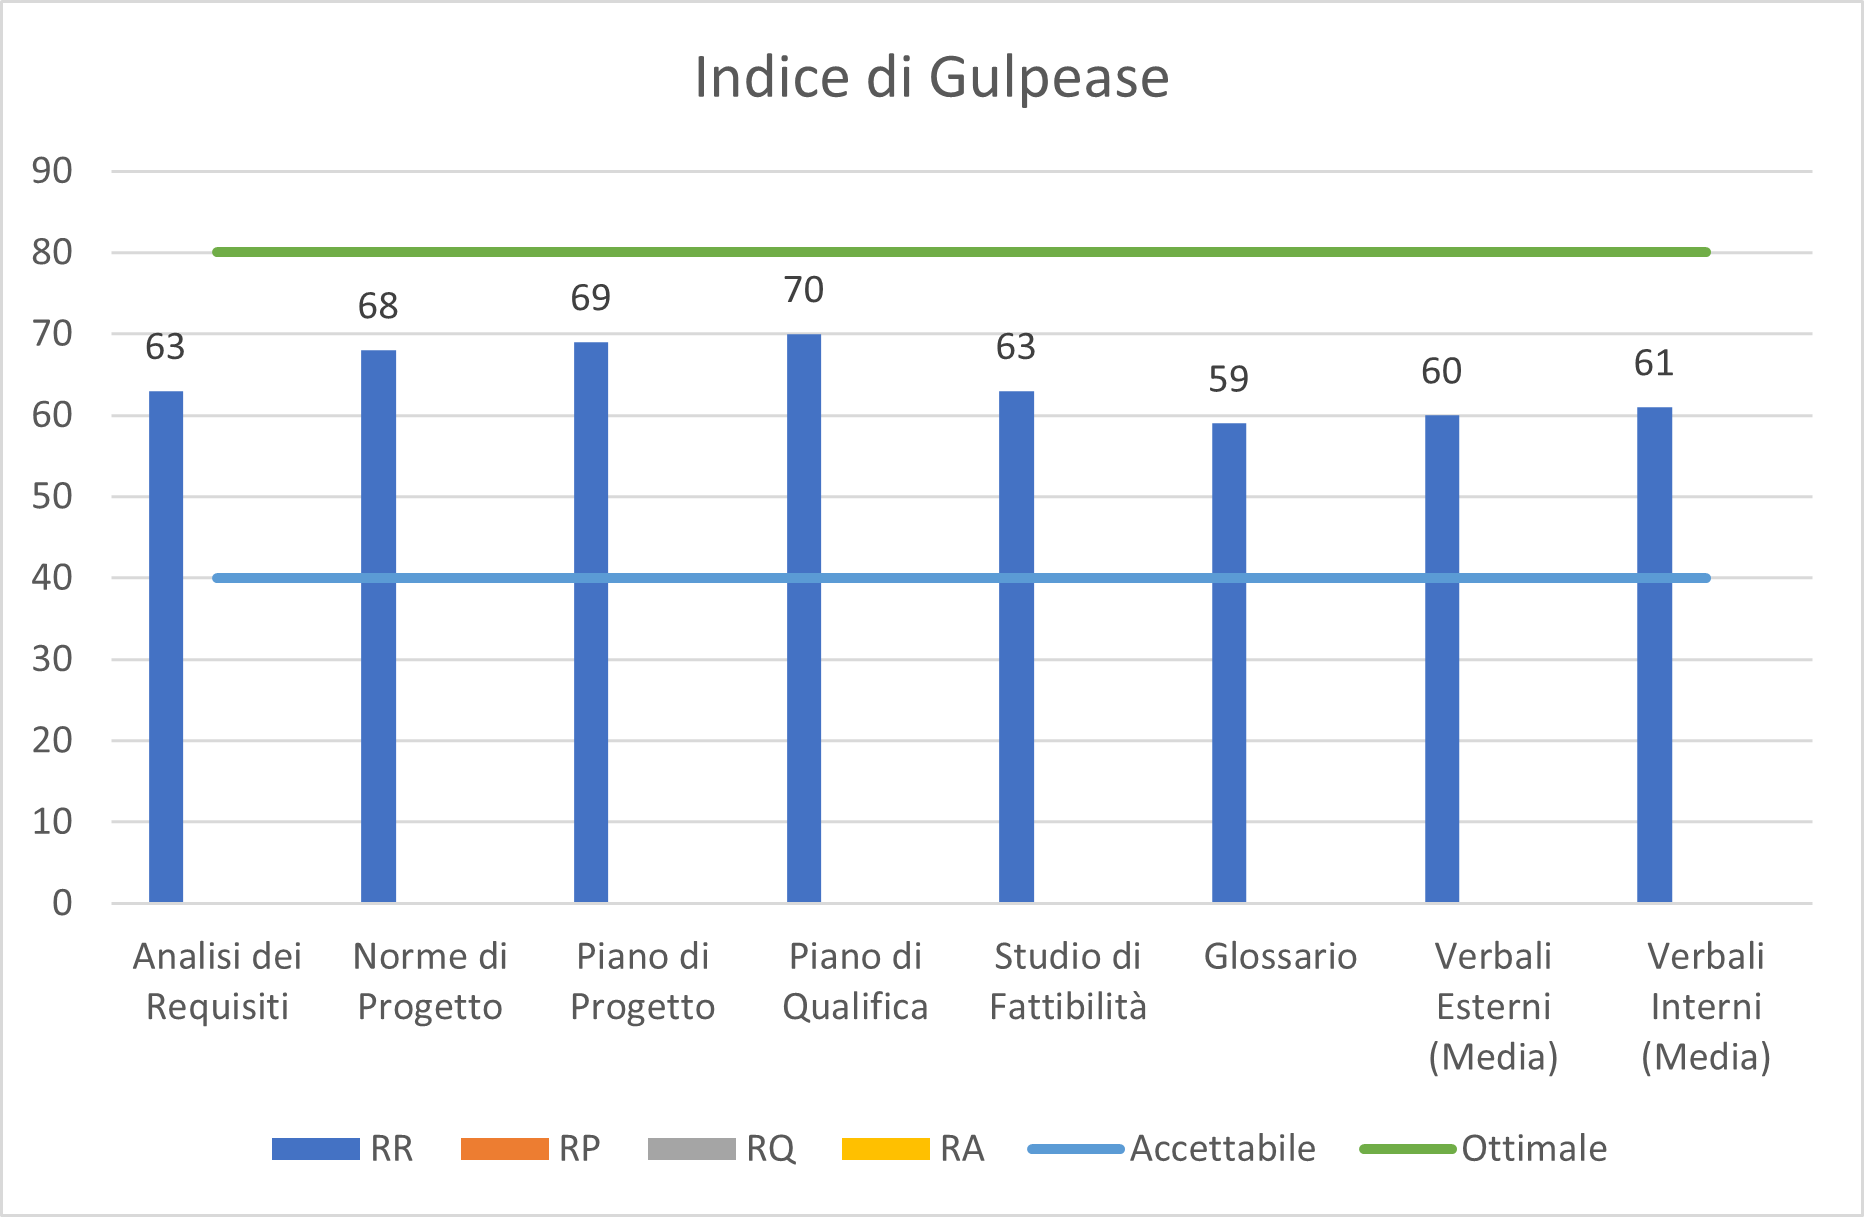
\includegraphics[scale=0.90]{res/ResocontoAttivitaDiVerifica/res/img/indiceGulpease.png}\\
\caption{Andamento complessivo dell'indice di Gulpease}
\end{figure}

\subsubsection{Grafico per documento}

\begin{figure}[H]
\centering
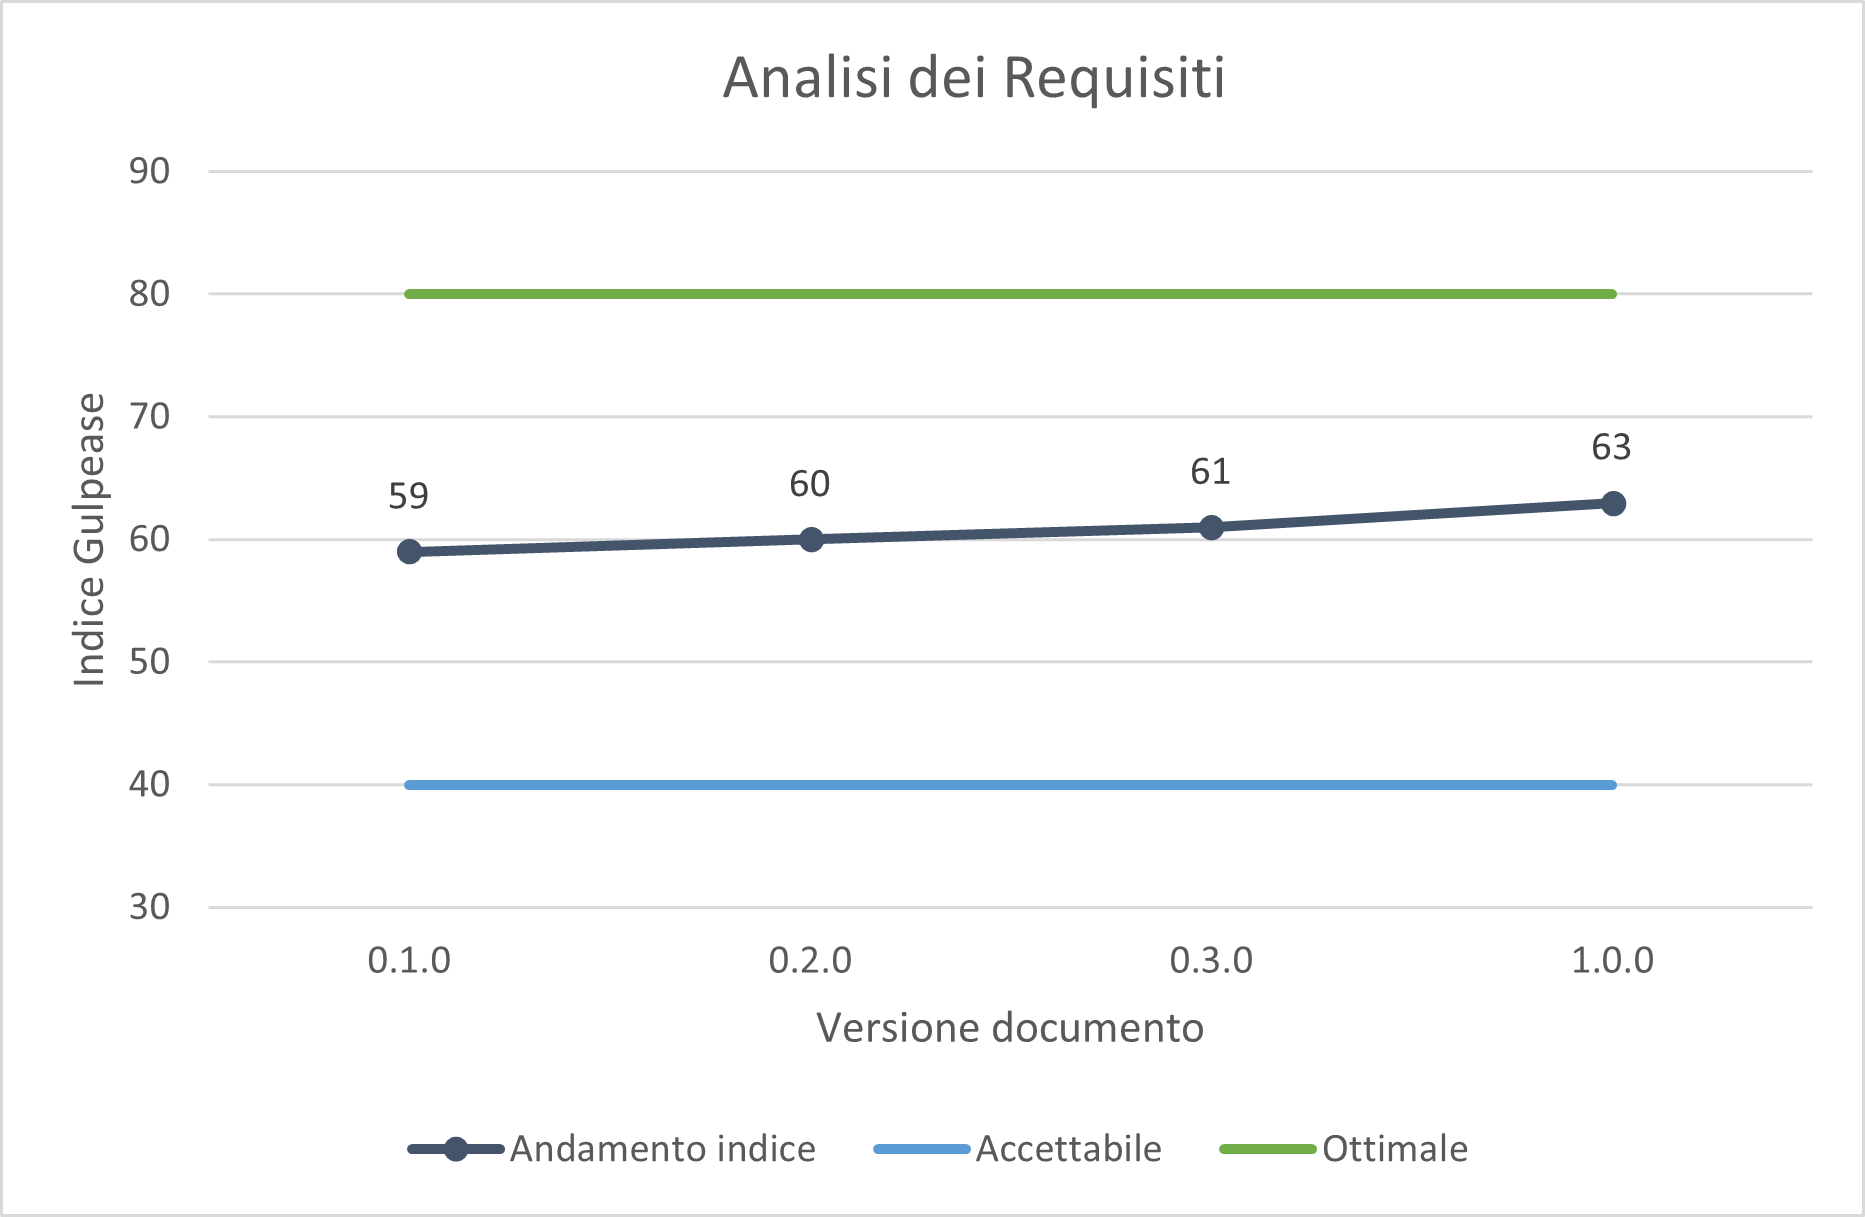
\includegraphics[scale=0.90]{res/ResocontoAttivitaDiVerifica/res/img/gulpeaseADR.png}\\
\caption{Andamento dell'indice di Gulpease \AdR}
\end{figure}

\begin{figure}[H]
\centering
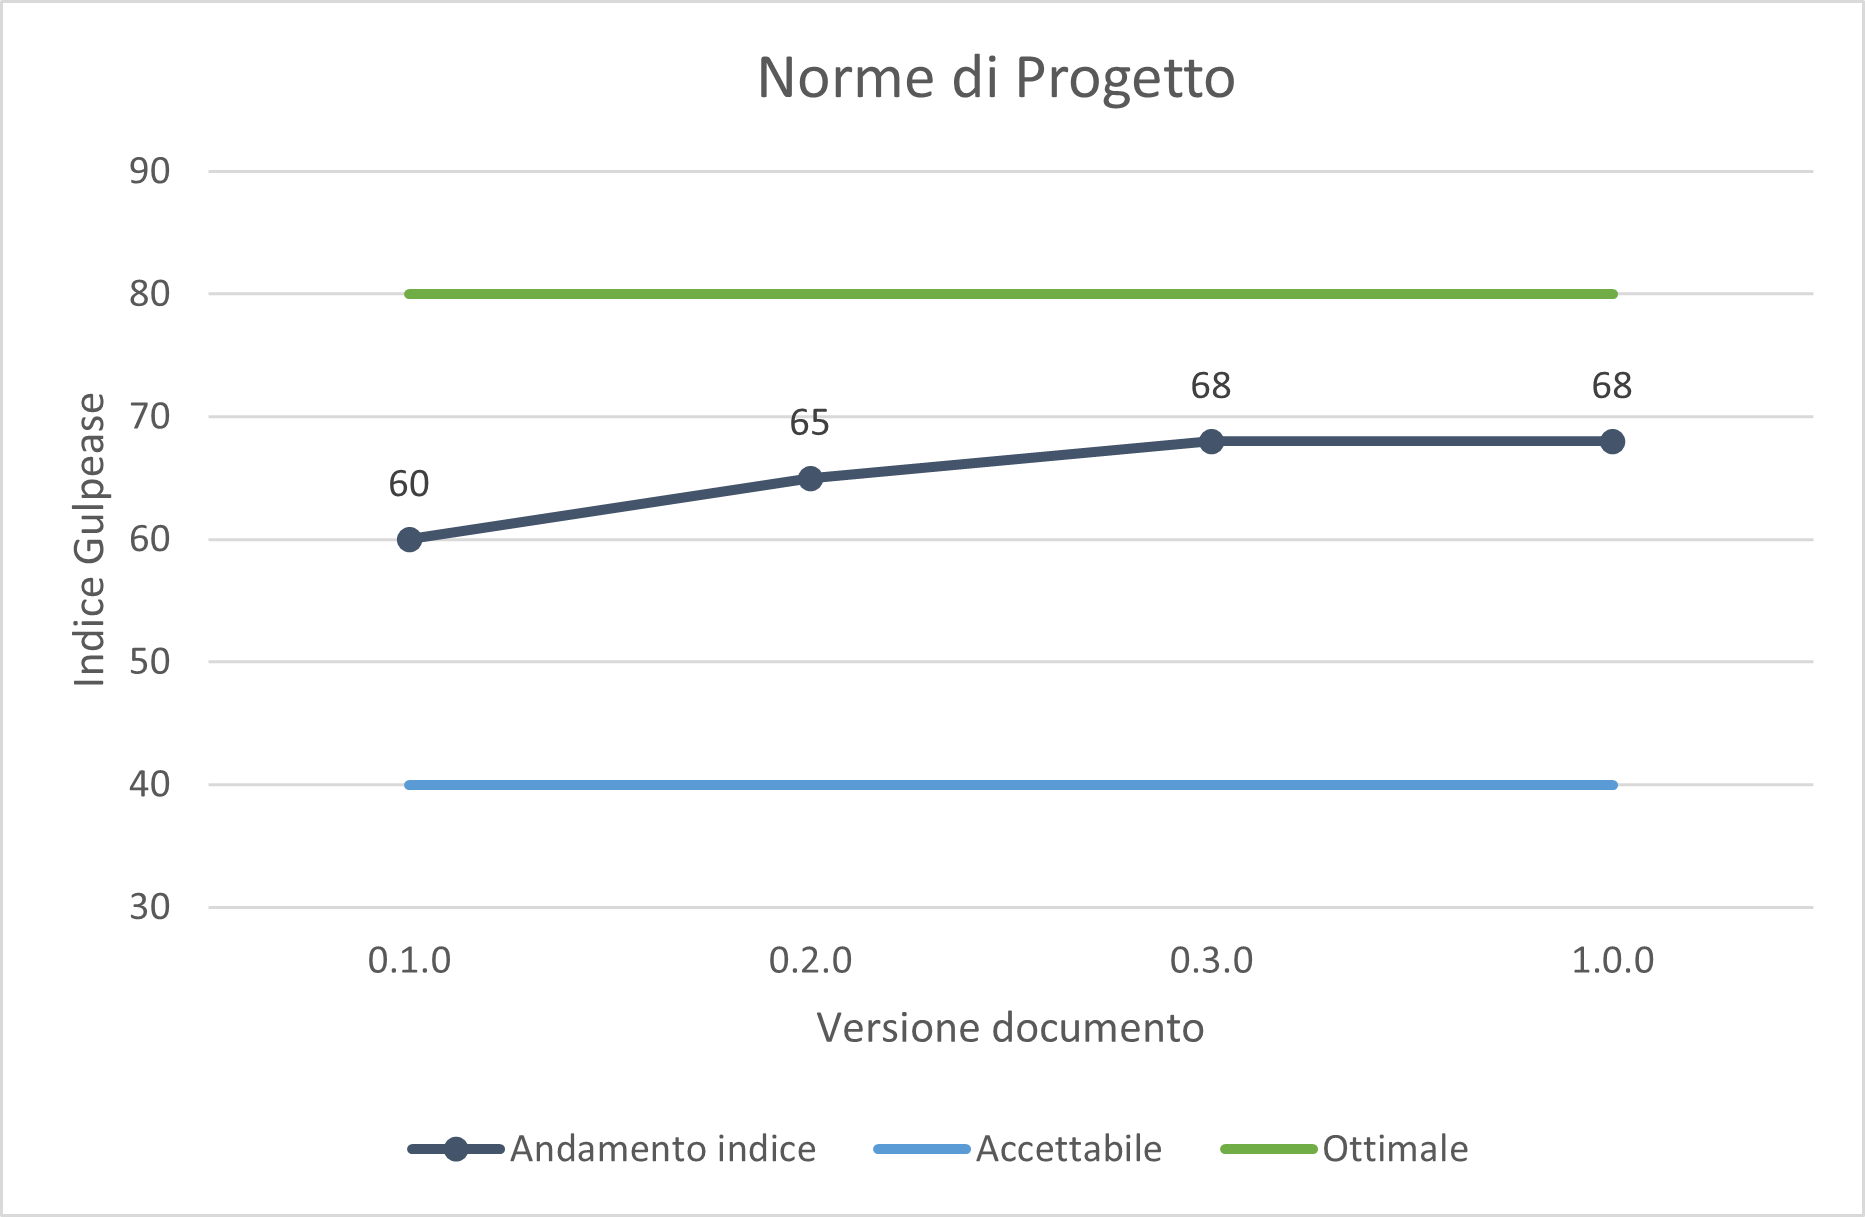
\includegraphics[scale=0.90]{res/ResocontoAttivitaDiVerifica/res/img/gulpeaseNDP.png}\\
\caption{Andamento dell'indice di Gulpease \NdP}
\end{figure}

\begin{figure}[H]
\centering
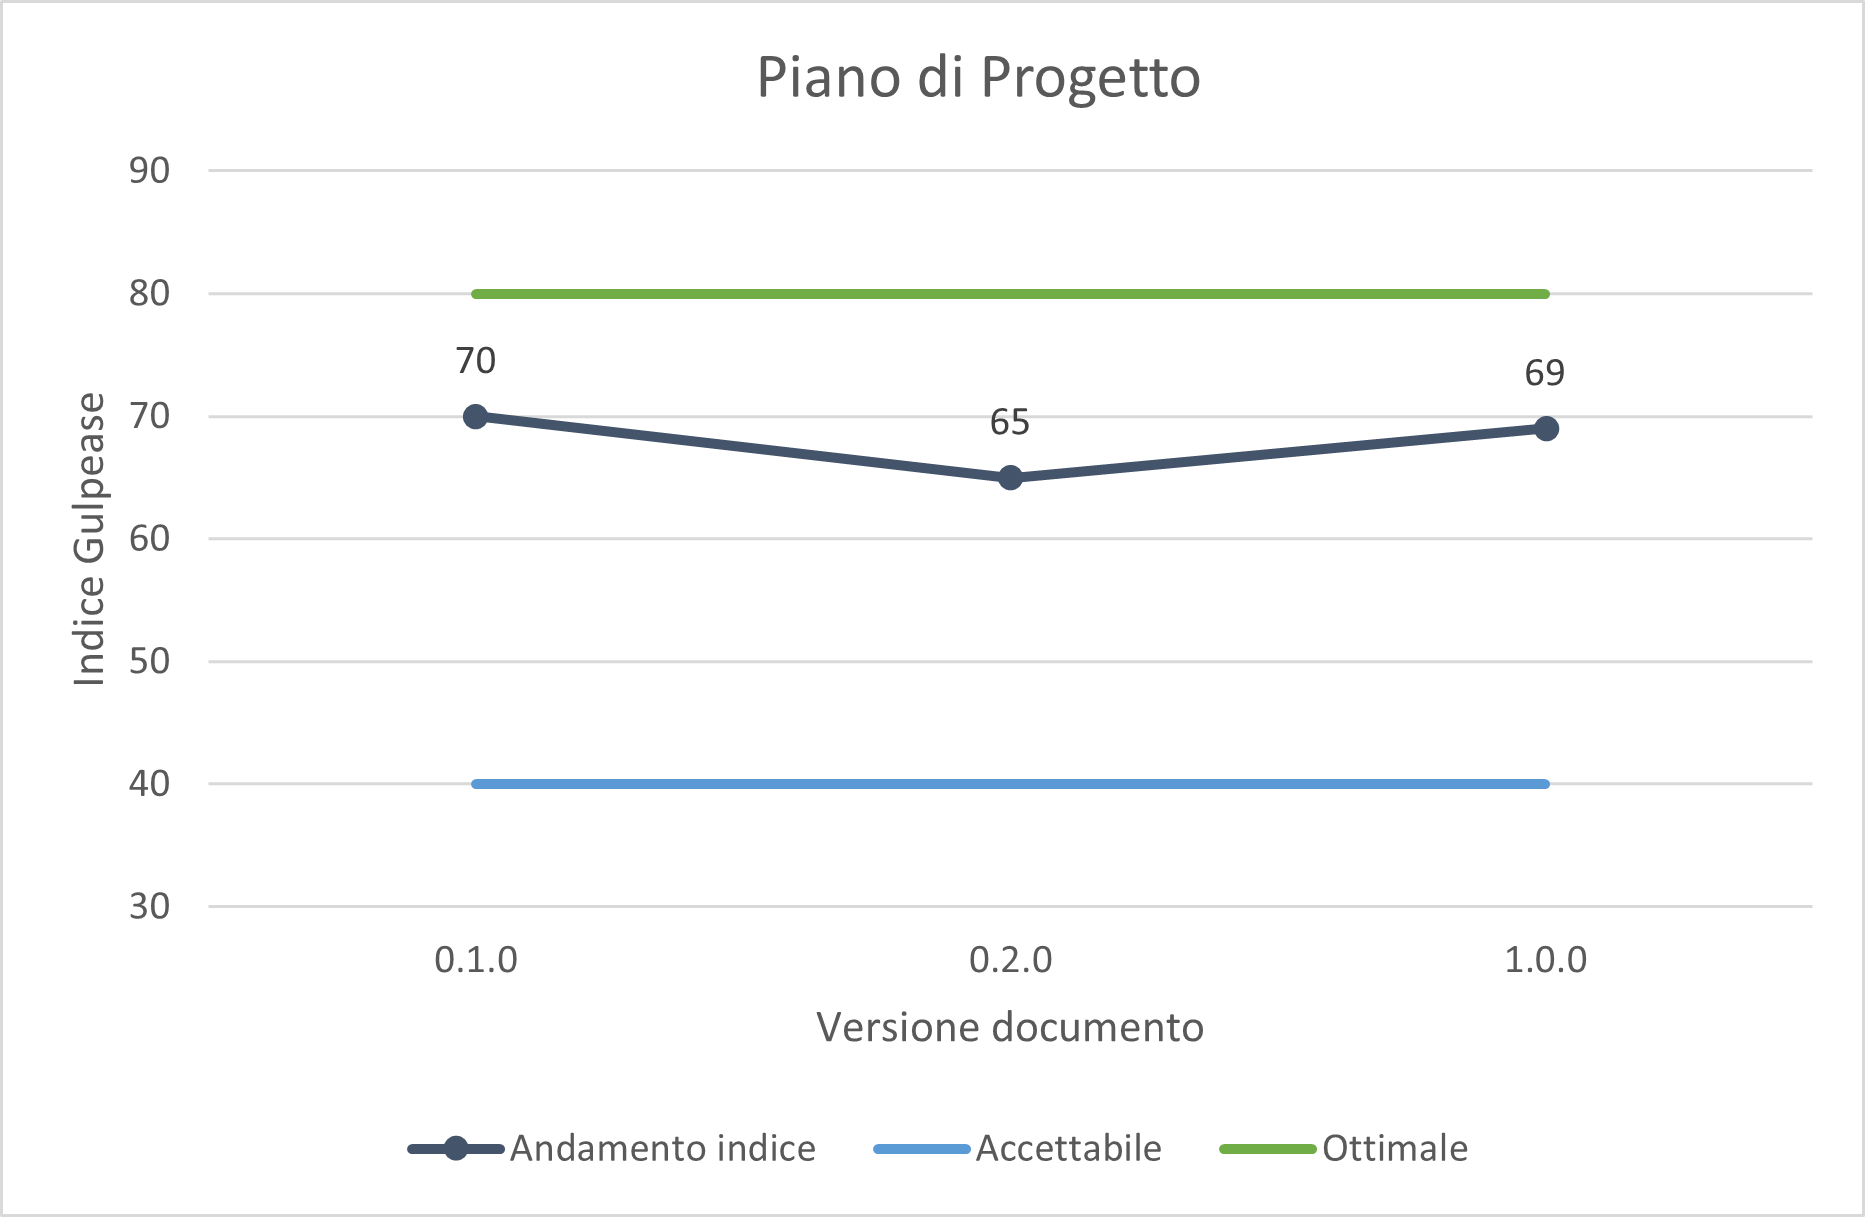
\includegraphics[scale=0.90]{res/ResocontoAttivitaDiVerifica/res/img/gulpeasePDP.png}\\
\caption{Andamento dell'indice di Gulpease \PdP}
\end{figure}

\begin{figure}[H]
\centering
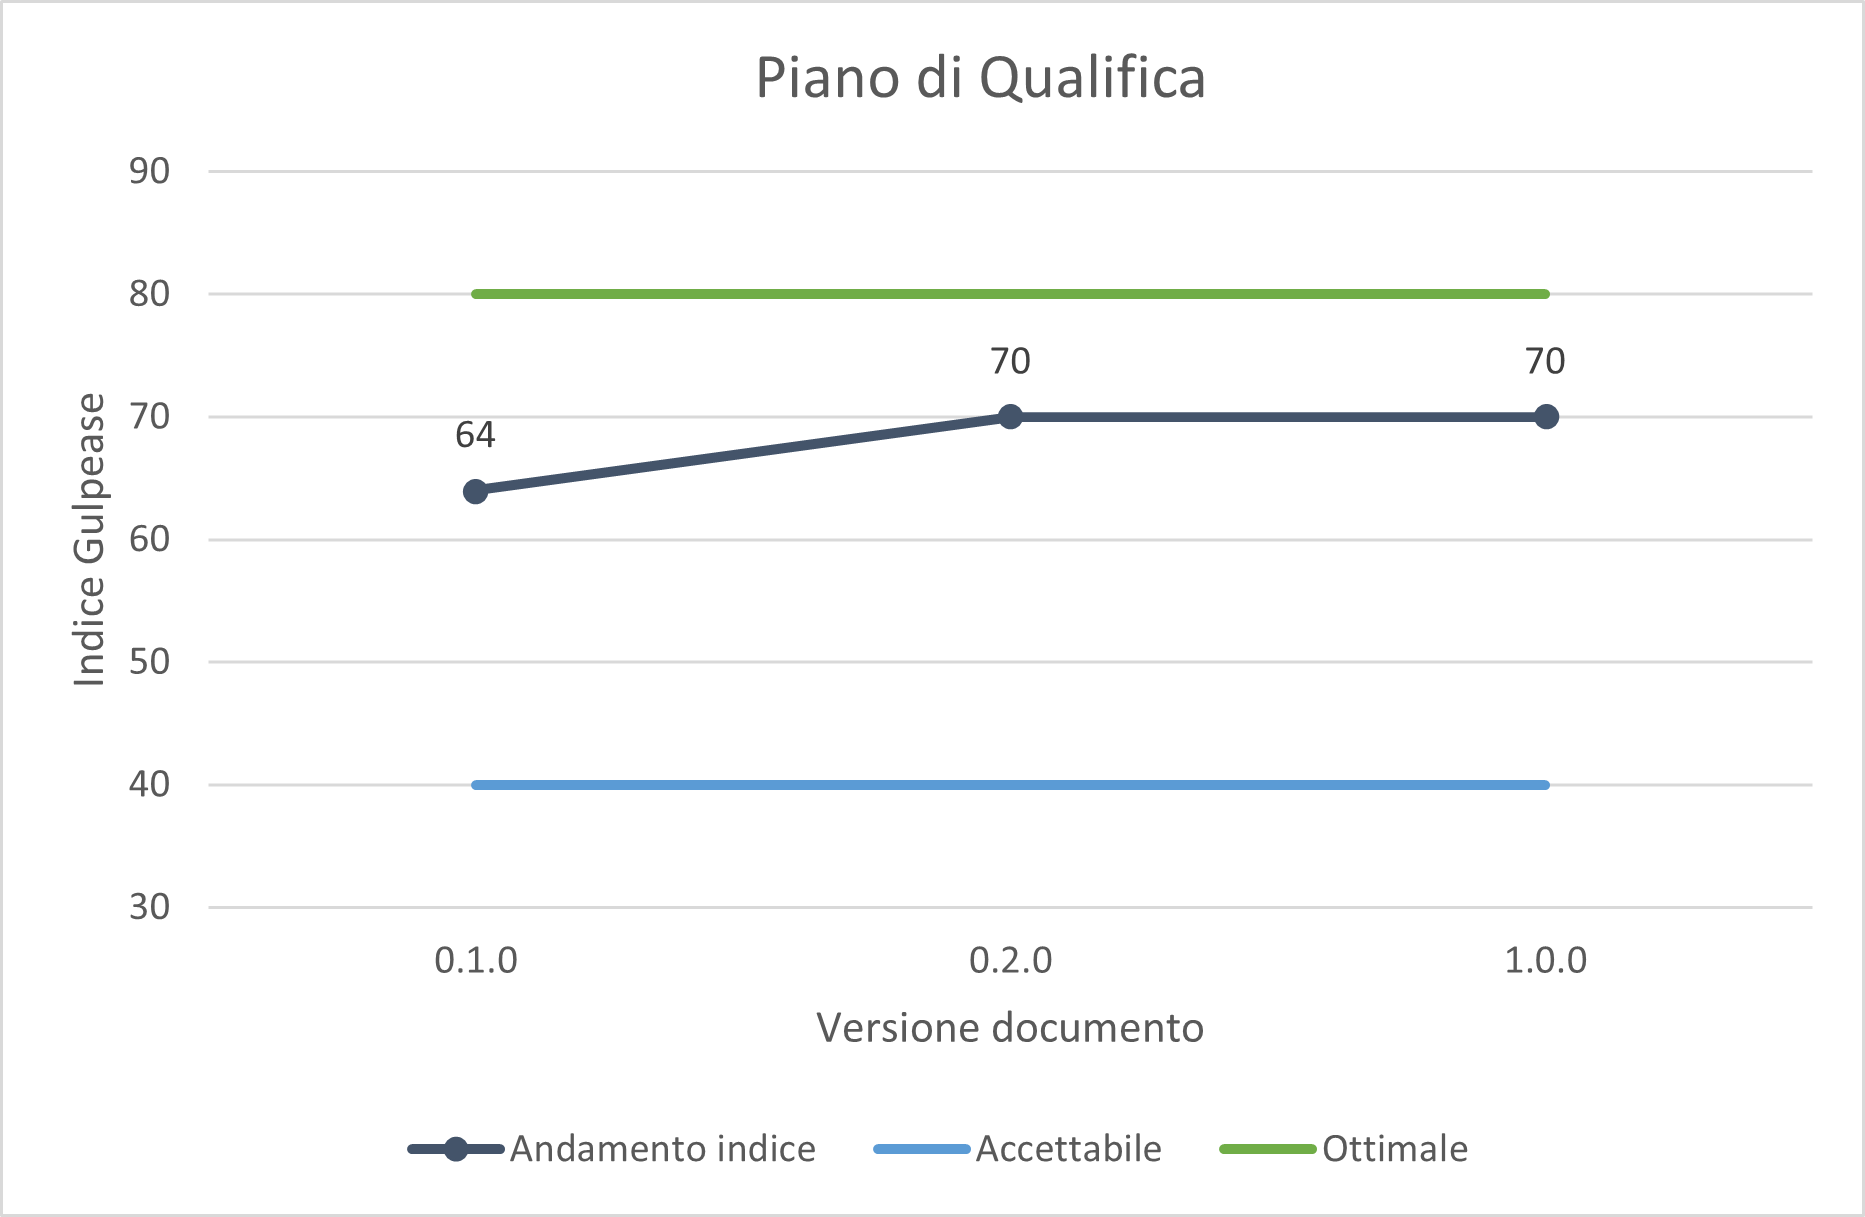
\includegraphics[scale=0.90]{res/ResocontoAttivitaDiVerifica/res/img/gulpeasePDQ.png}\\
\caption{Andamento dell'indice di Gulpease \PdQ}
\end{figure}

\begin{figure}[H]
\centering
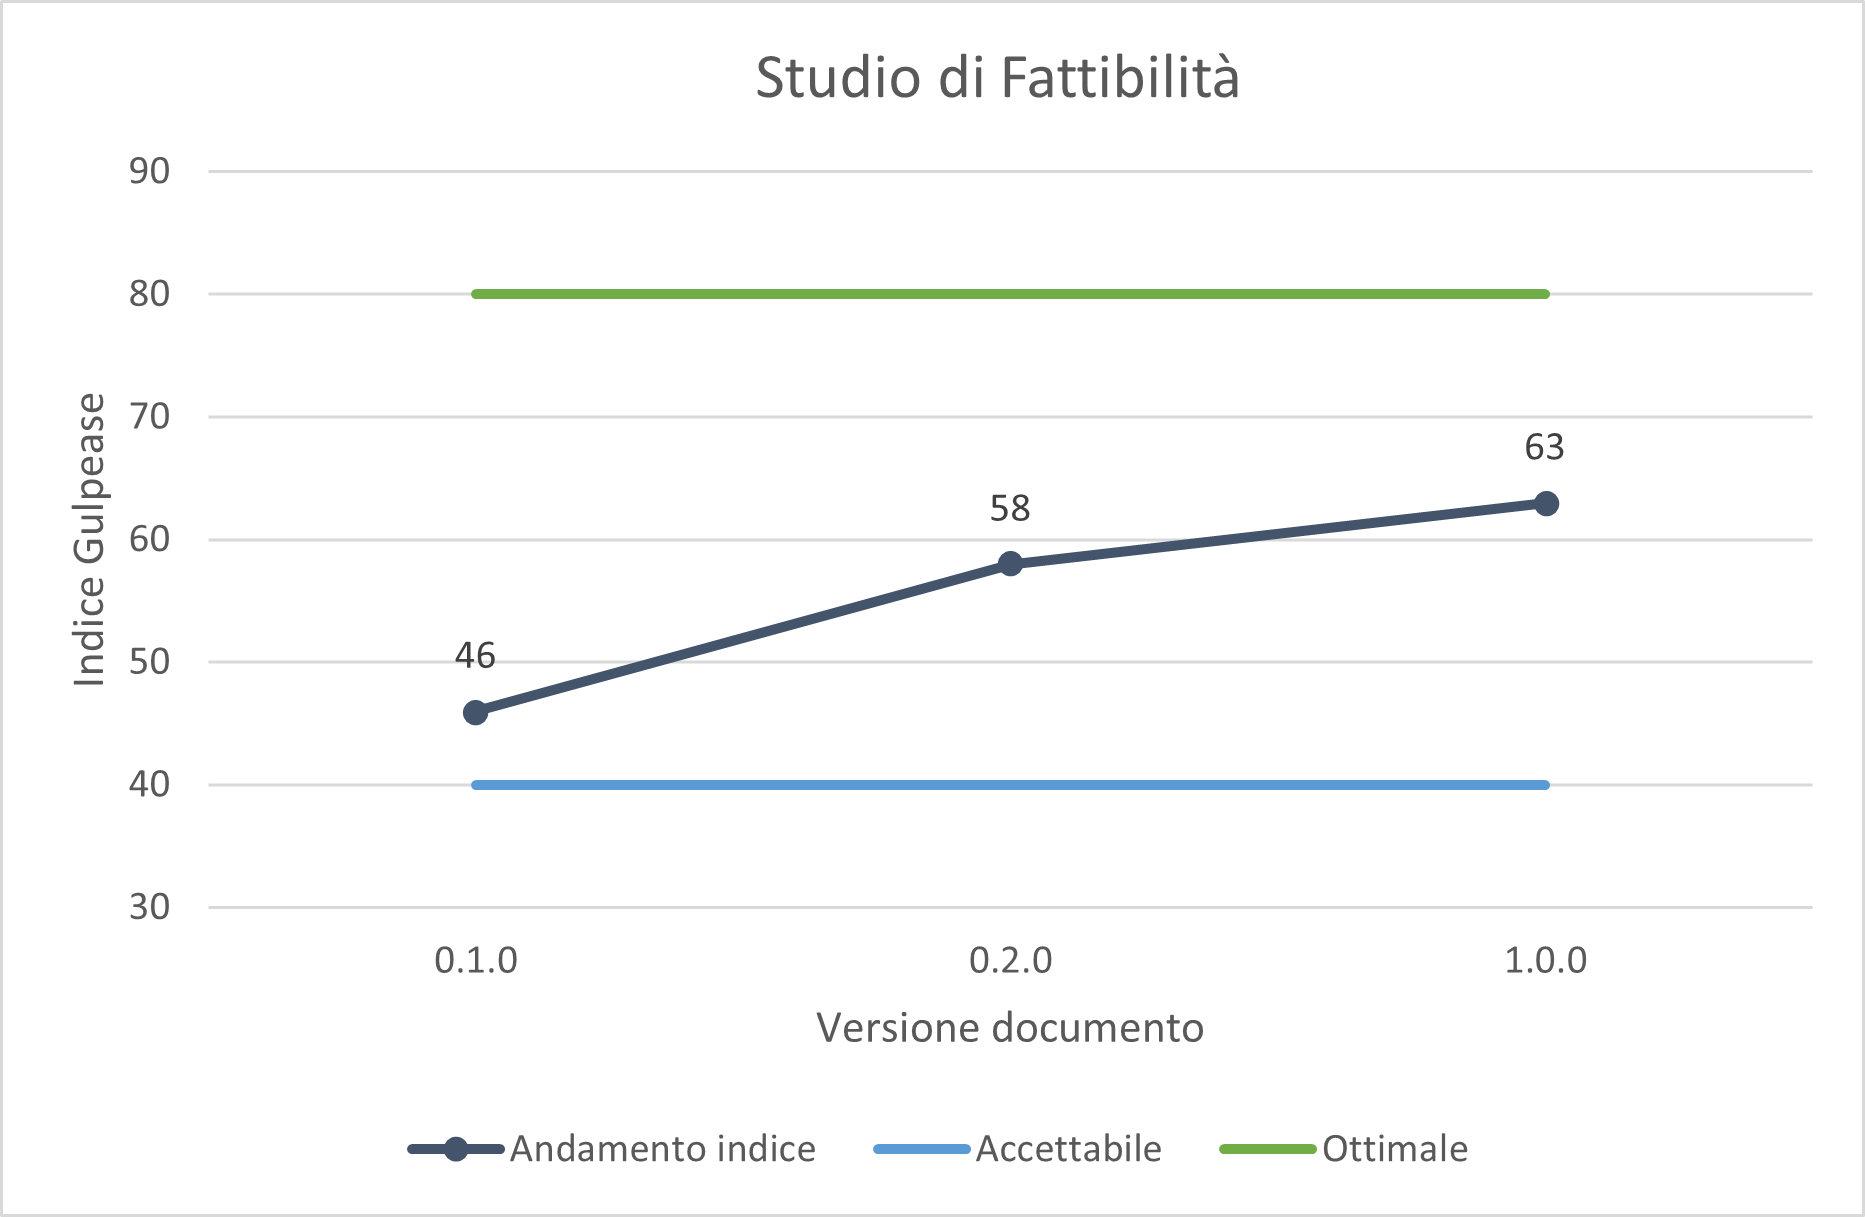
\includegraphics[scale=0.90]{res/ResocontoAttivitaDiVerifica/res/img/gulpeaseSDF.png}\\
\caption{Andamento dell'indice di Gulpease \SdF}
\end{figure}

\begin{figure}[H]
\centering
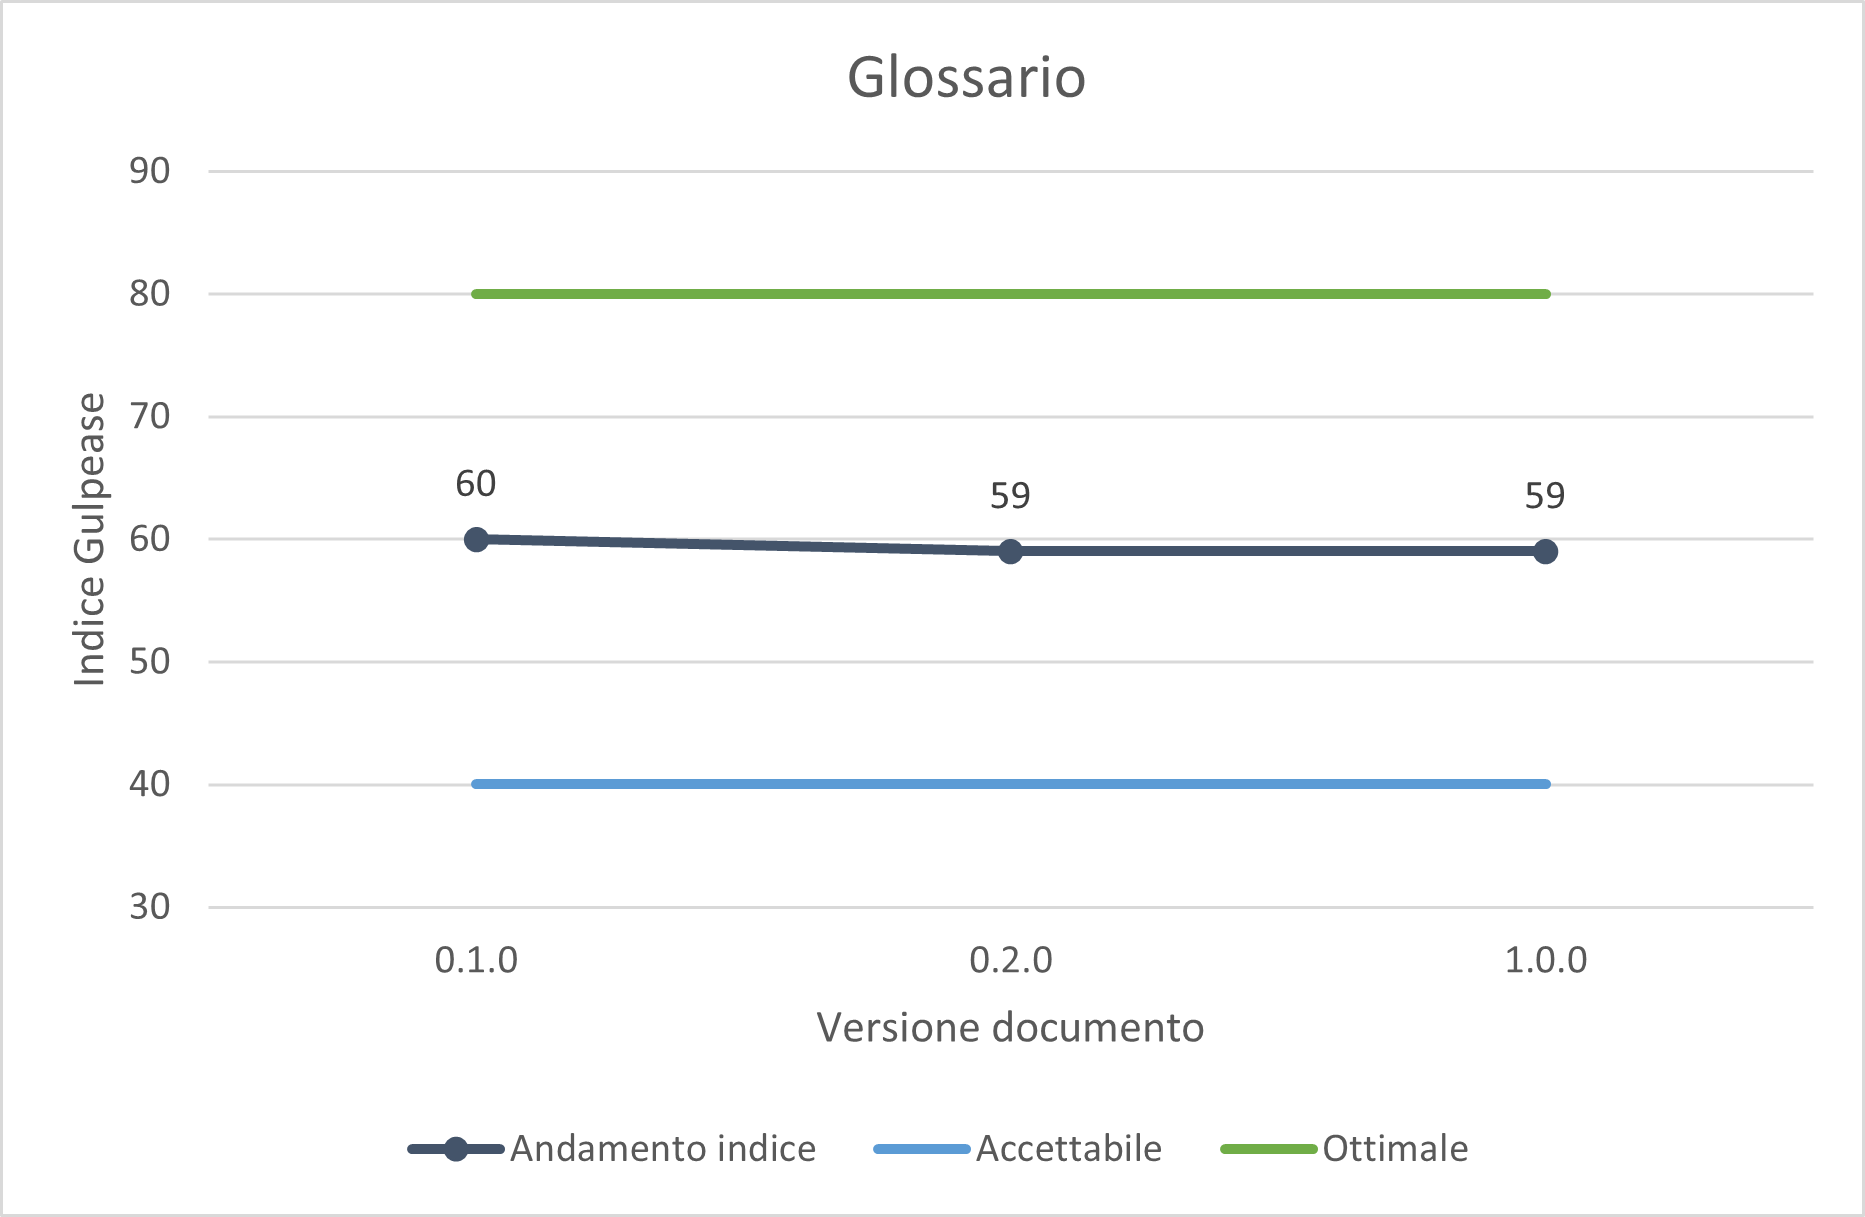
\includegraphics[scale=0.90]{res/ResocontoAttivitaDiVerifica/res/img/gulpeaseG.png}\\
\caption{Andamento dell'indice di Gulpease \Glossario}
\end{figure}



\subsubsection{MPC4 - Correttezza ortografica}
Di seguito è riportato il grafico degli errori ortografici rilevati sui vari documenti, il cui valore è definito accettabile e ottimale come descritto nella sezione §2.2.1.2.\\

\begin{figure}[H]
\centering
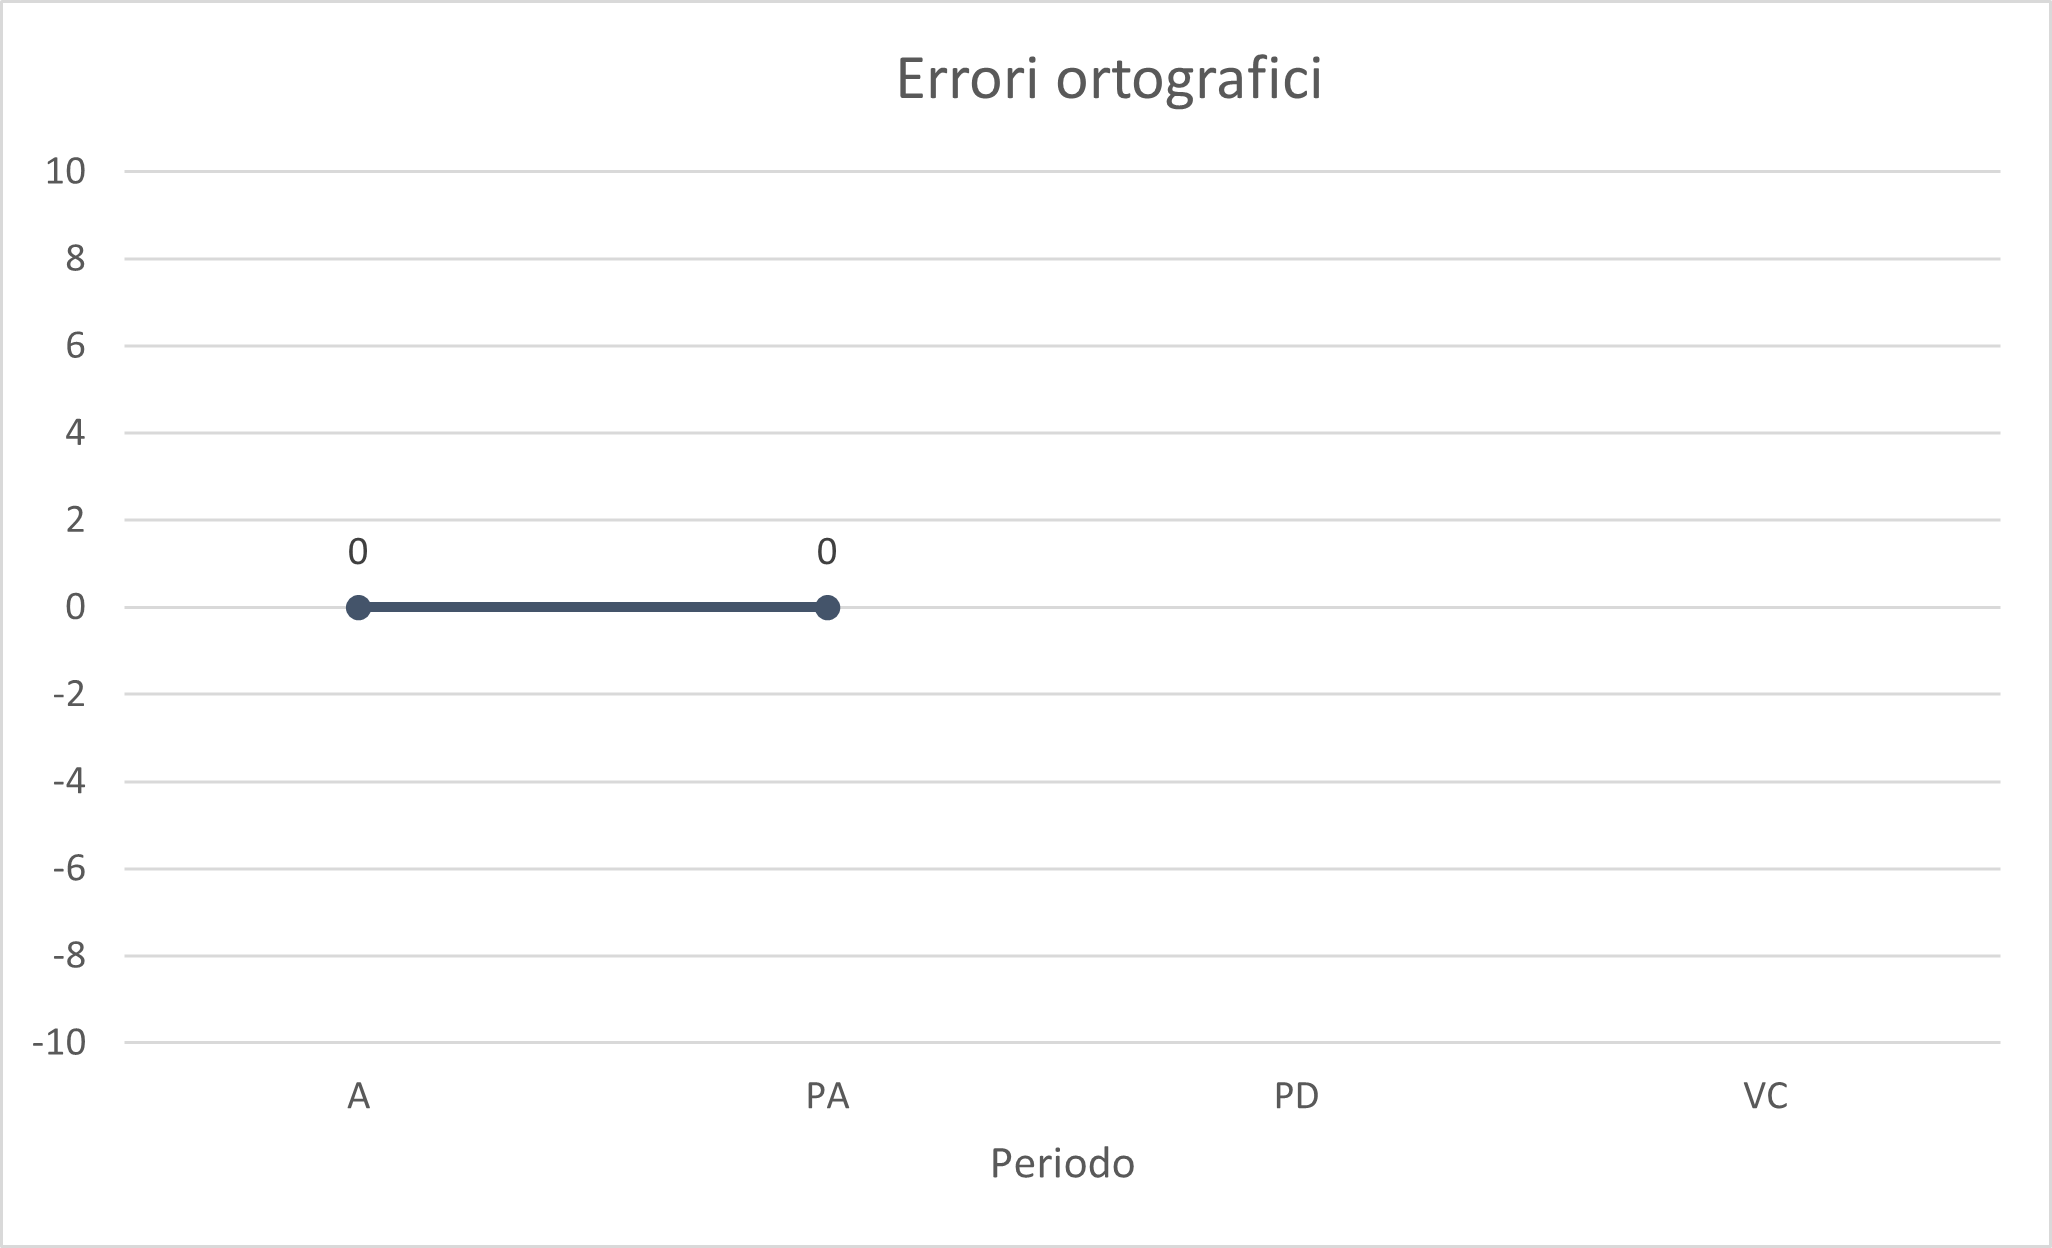
\includegraphics[scale=0.78]{res/ResocontoAttivitaDiVerifica/res/metriche/grafici/img/correttezzaOrtografica.png}\\
\caption{Andamento della correttezza ortografica}
\end{figure}

\subsubsection{MPC6 - Estimate at Completion}
Di seguito è riportato il grafico dell'Estimate at Completion, il cui valore è definito accettabile e ottimale come descritto nella sezione §2.3.1.1.\\

\begin{figure}[H]
\centering
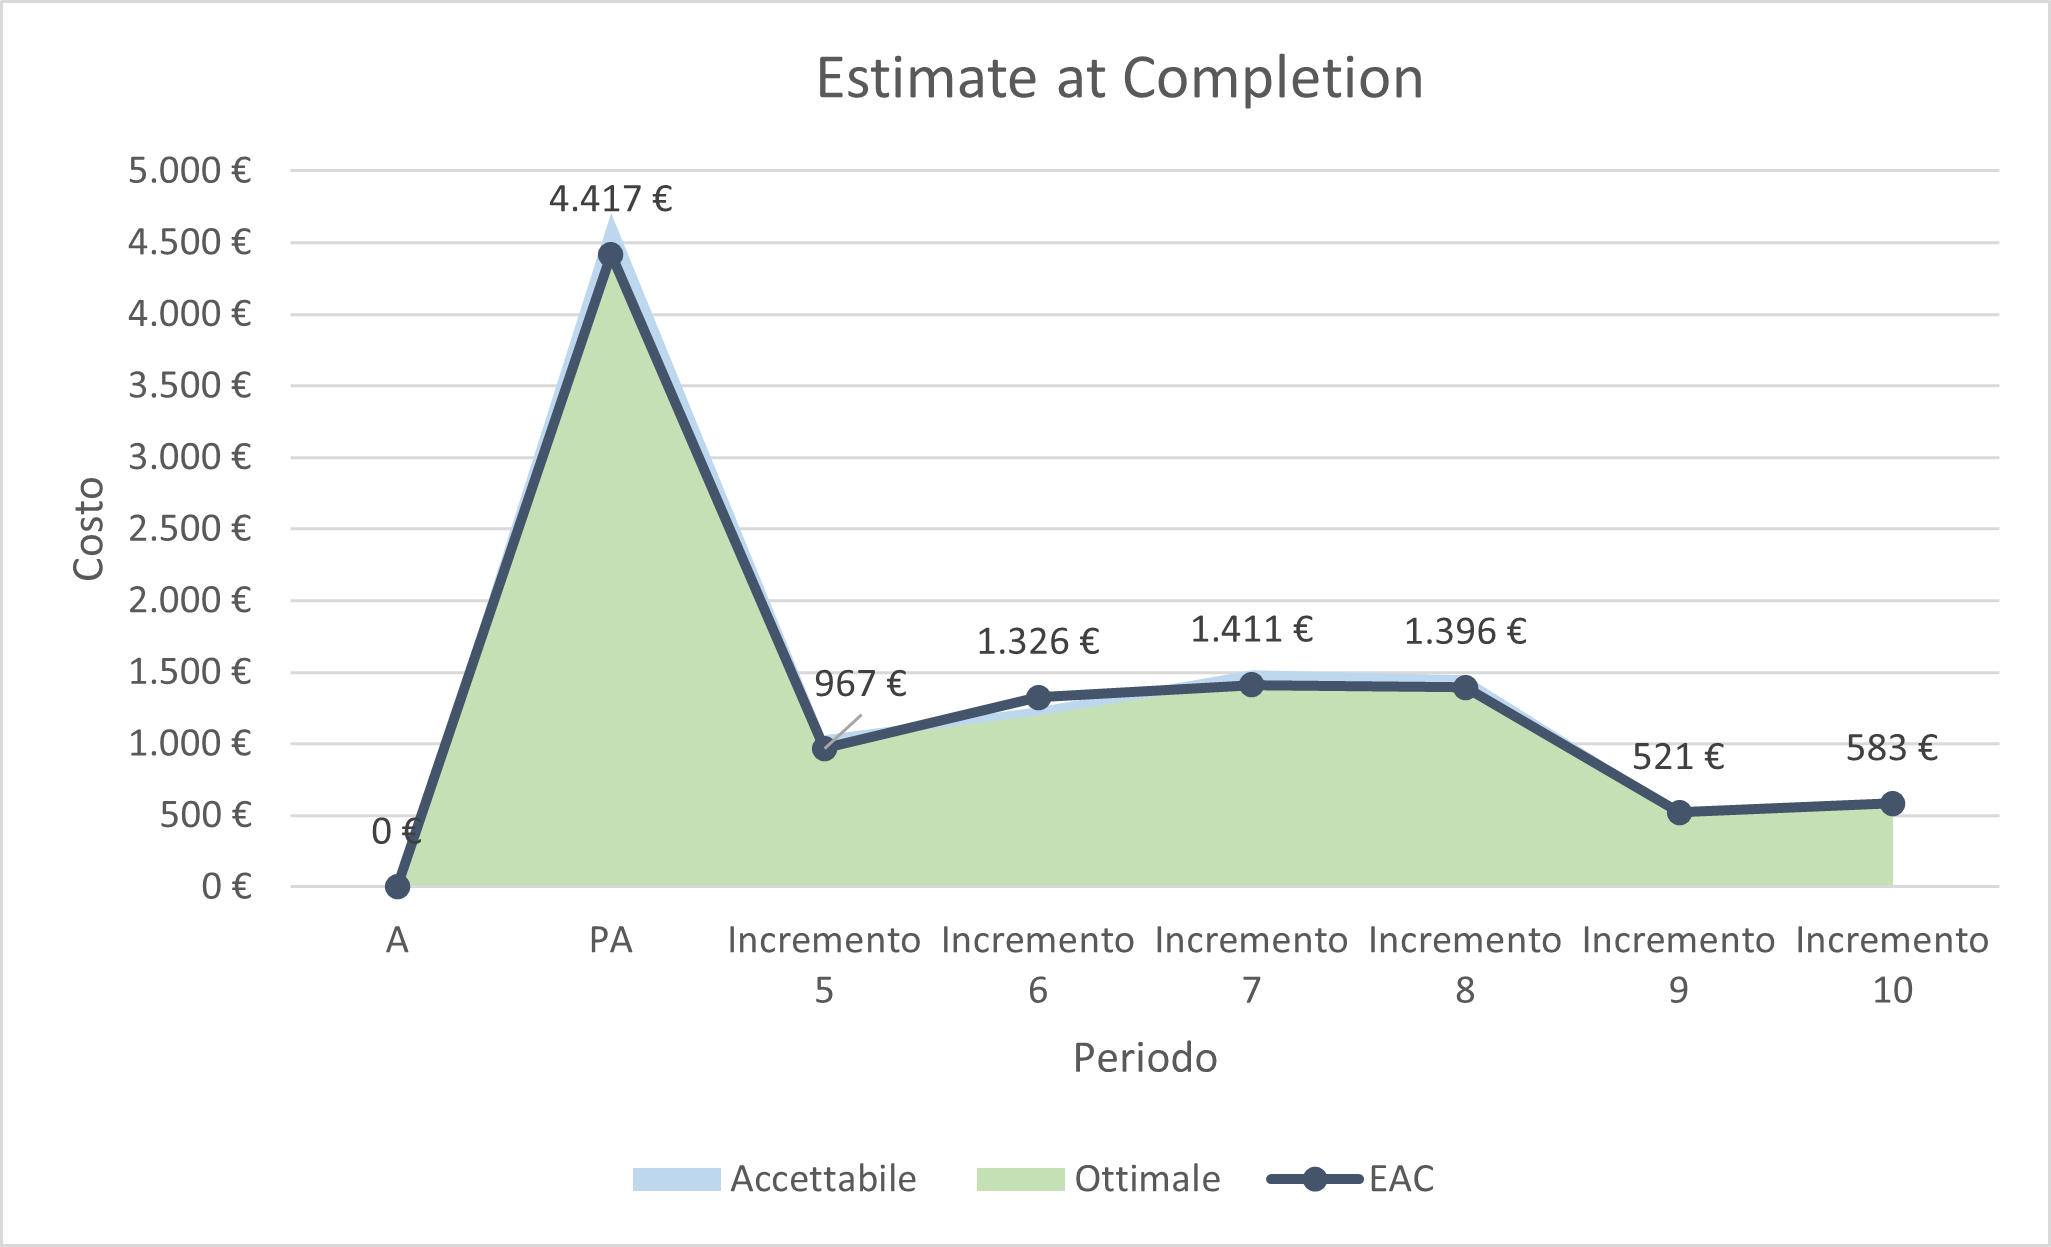
\includegraphics[scale=0.78]{res/ResocontoAttivitaDiVerifica/res/metriche/grafici/img/estimateCompletion.png}\\
\caption{Andamento Estimate at Completion}
\end{figure}

\subsubsection{MPC7 - Variance at Completion}
Di seguito è riportato il grafico della Variance at Completion, il cui valore è definito accettabile e ottimale come descritto nella sezione §2.3.1.2.\\

\begin{figure}[H]
\centering
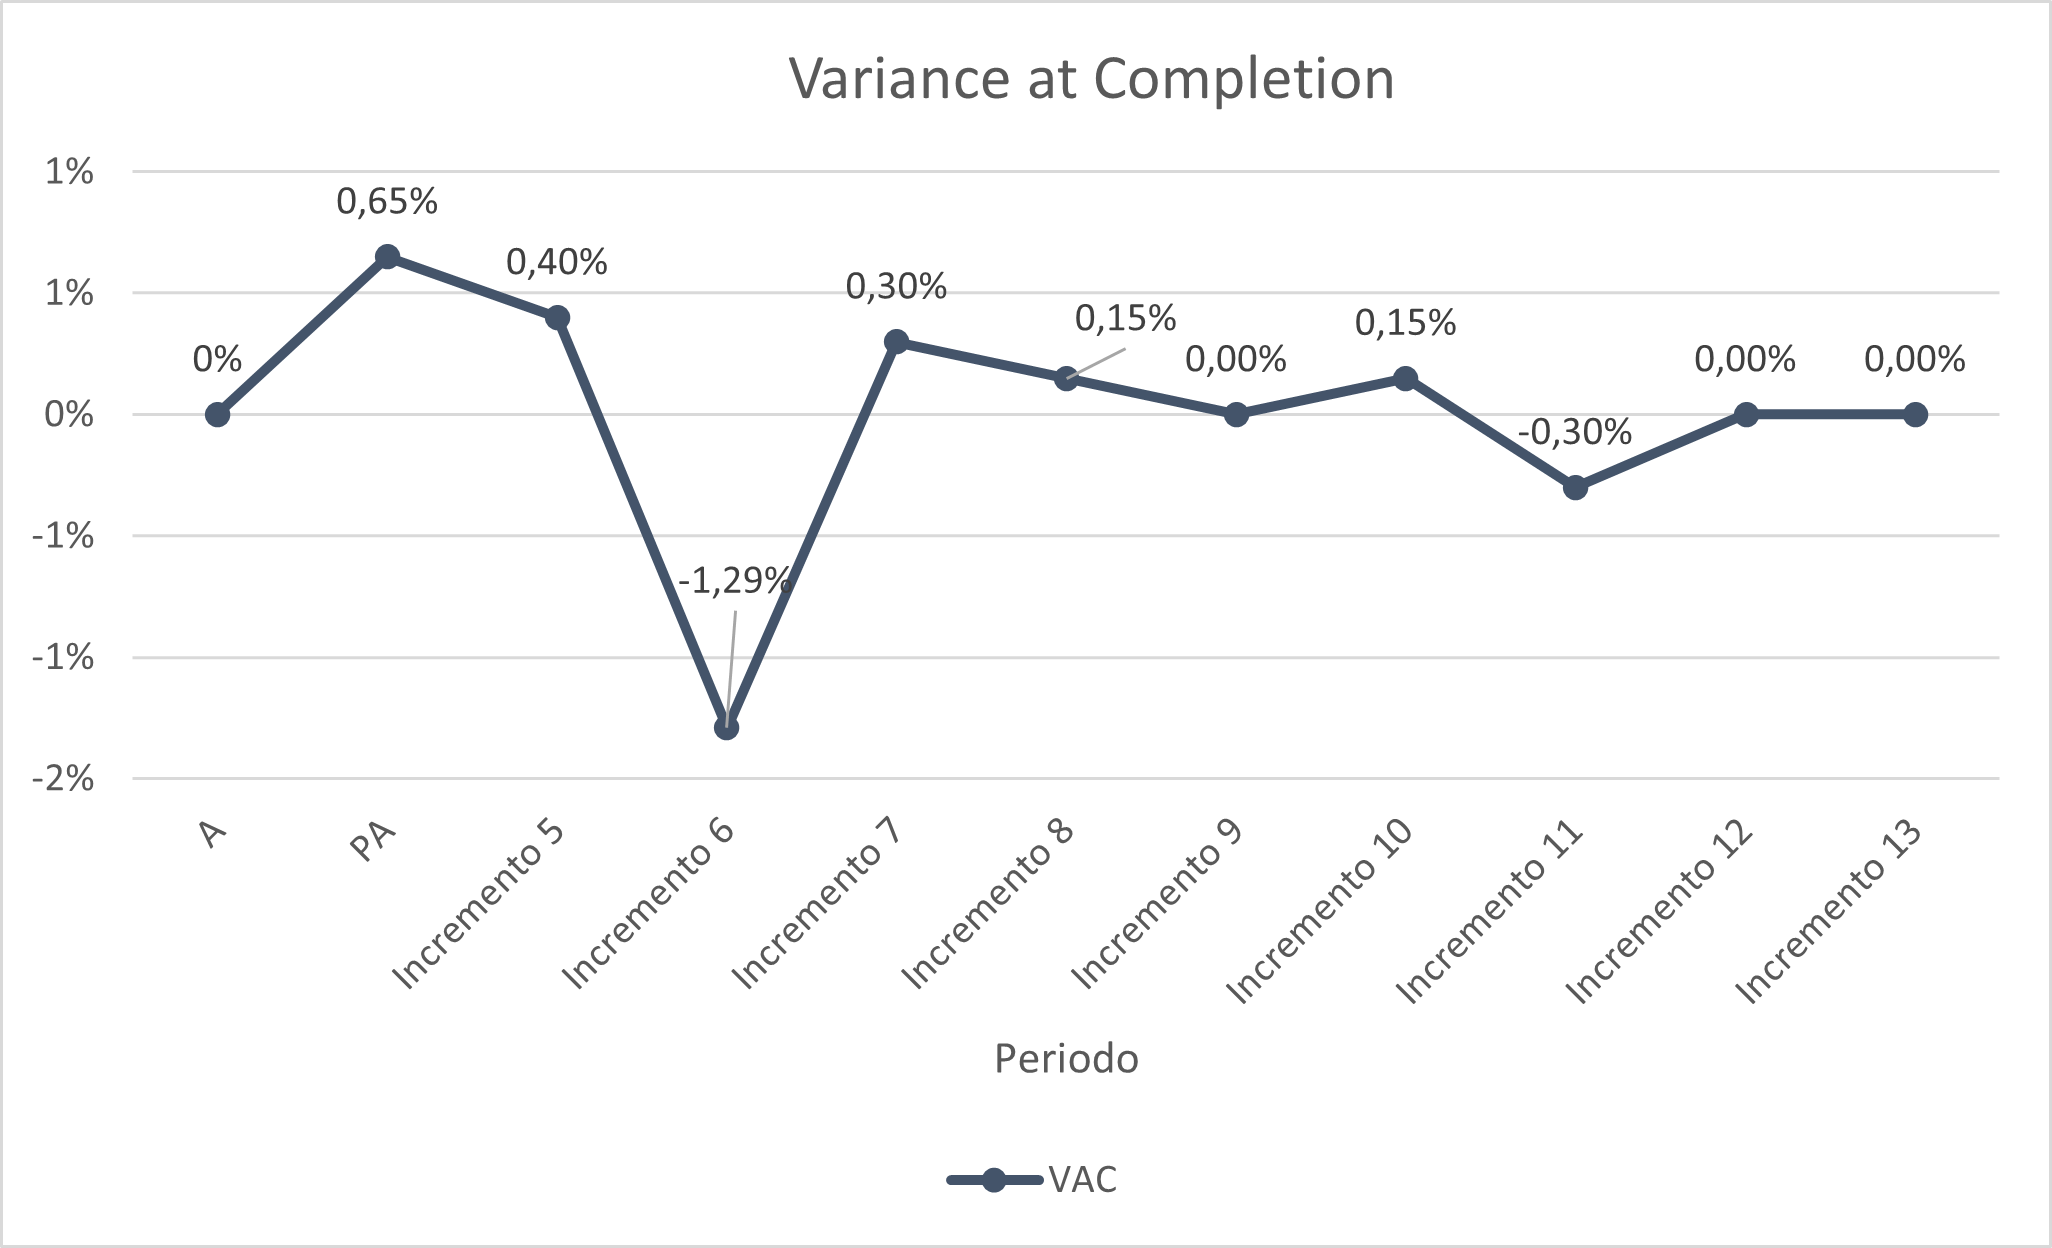
\includegraphics[scale=0.78]{res/ResocontoAttivitaDiVerifica/res/metriche/grafici/img/varianceCompletion.png}\\
\caption{Andamento Variance at Completion}
\end{figure}

\subsubsection{MPC8 - Actual Cost}
Di seguito è riportato il grafico dell'Actual Cost, il cui valore è definito accettabile e ottimale come descritto nella sezione §2.3.1.3.\\

\begin{figure}[H]
\centering
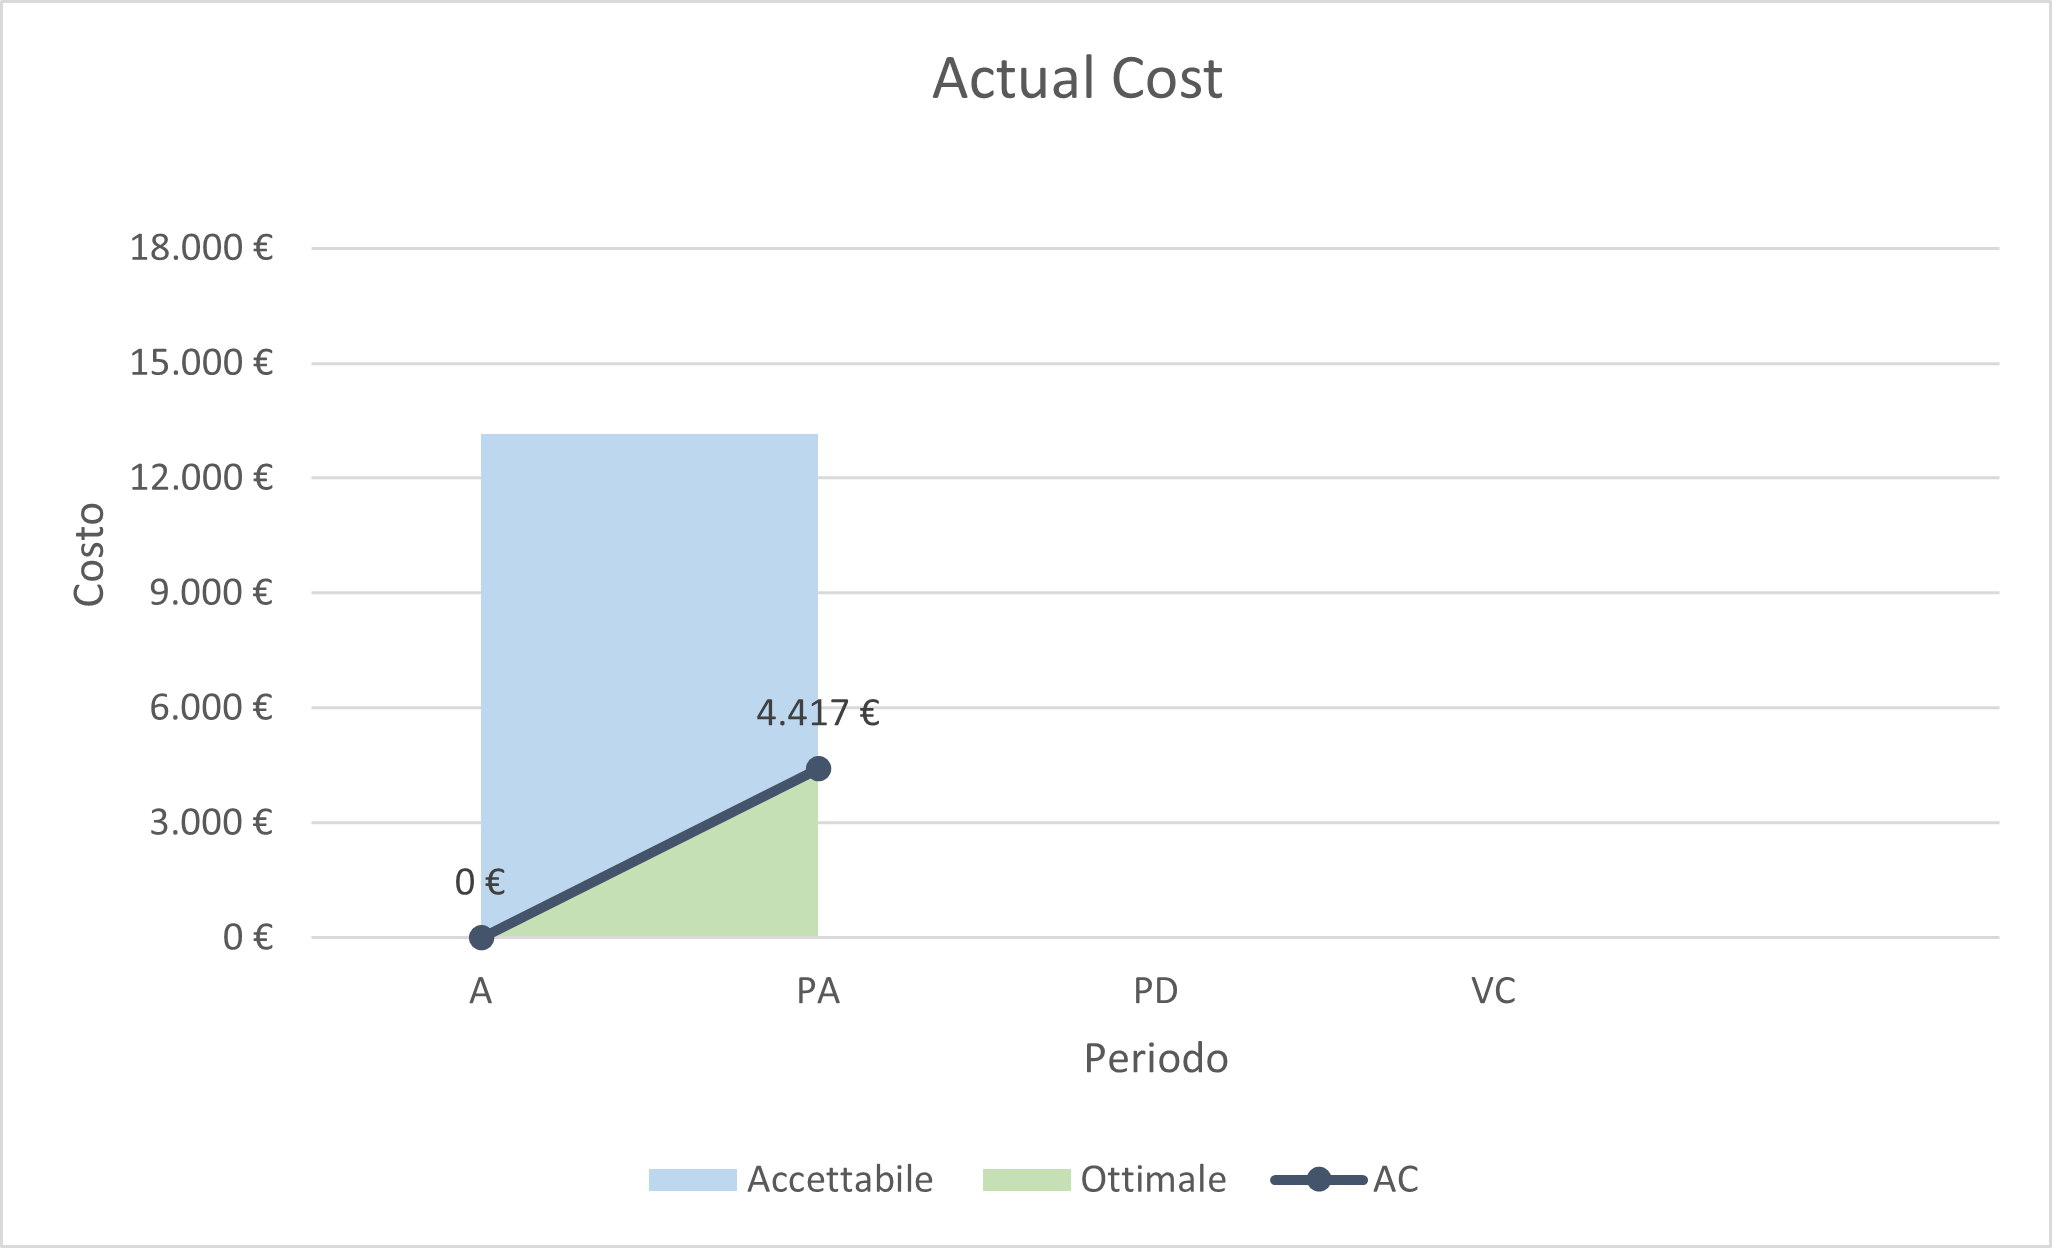
\includegraphics[scale=0.78]{res/ResocontoAttivitaDiVerifica/res/metriche/grafici/img/actualCost.png}\\
\caption{Andamento Actual Cost}
\end{figure}

\subsubsection{MPC10 - Budget Variance}
Di seguito è riportato il grafico del Budget Variance, il cui valore è definito accettabile e ottimale come descritto nella sezione §2.3.1.4.\\

\begin{figure}[H]
\centering
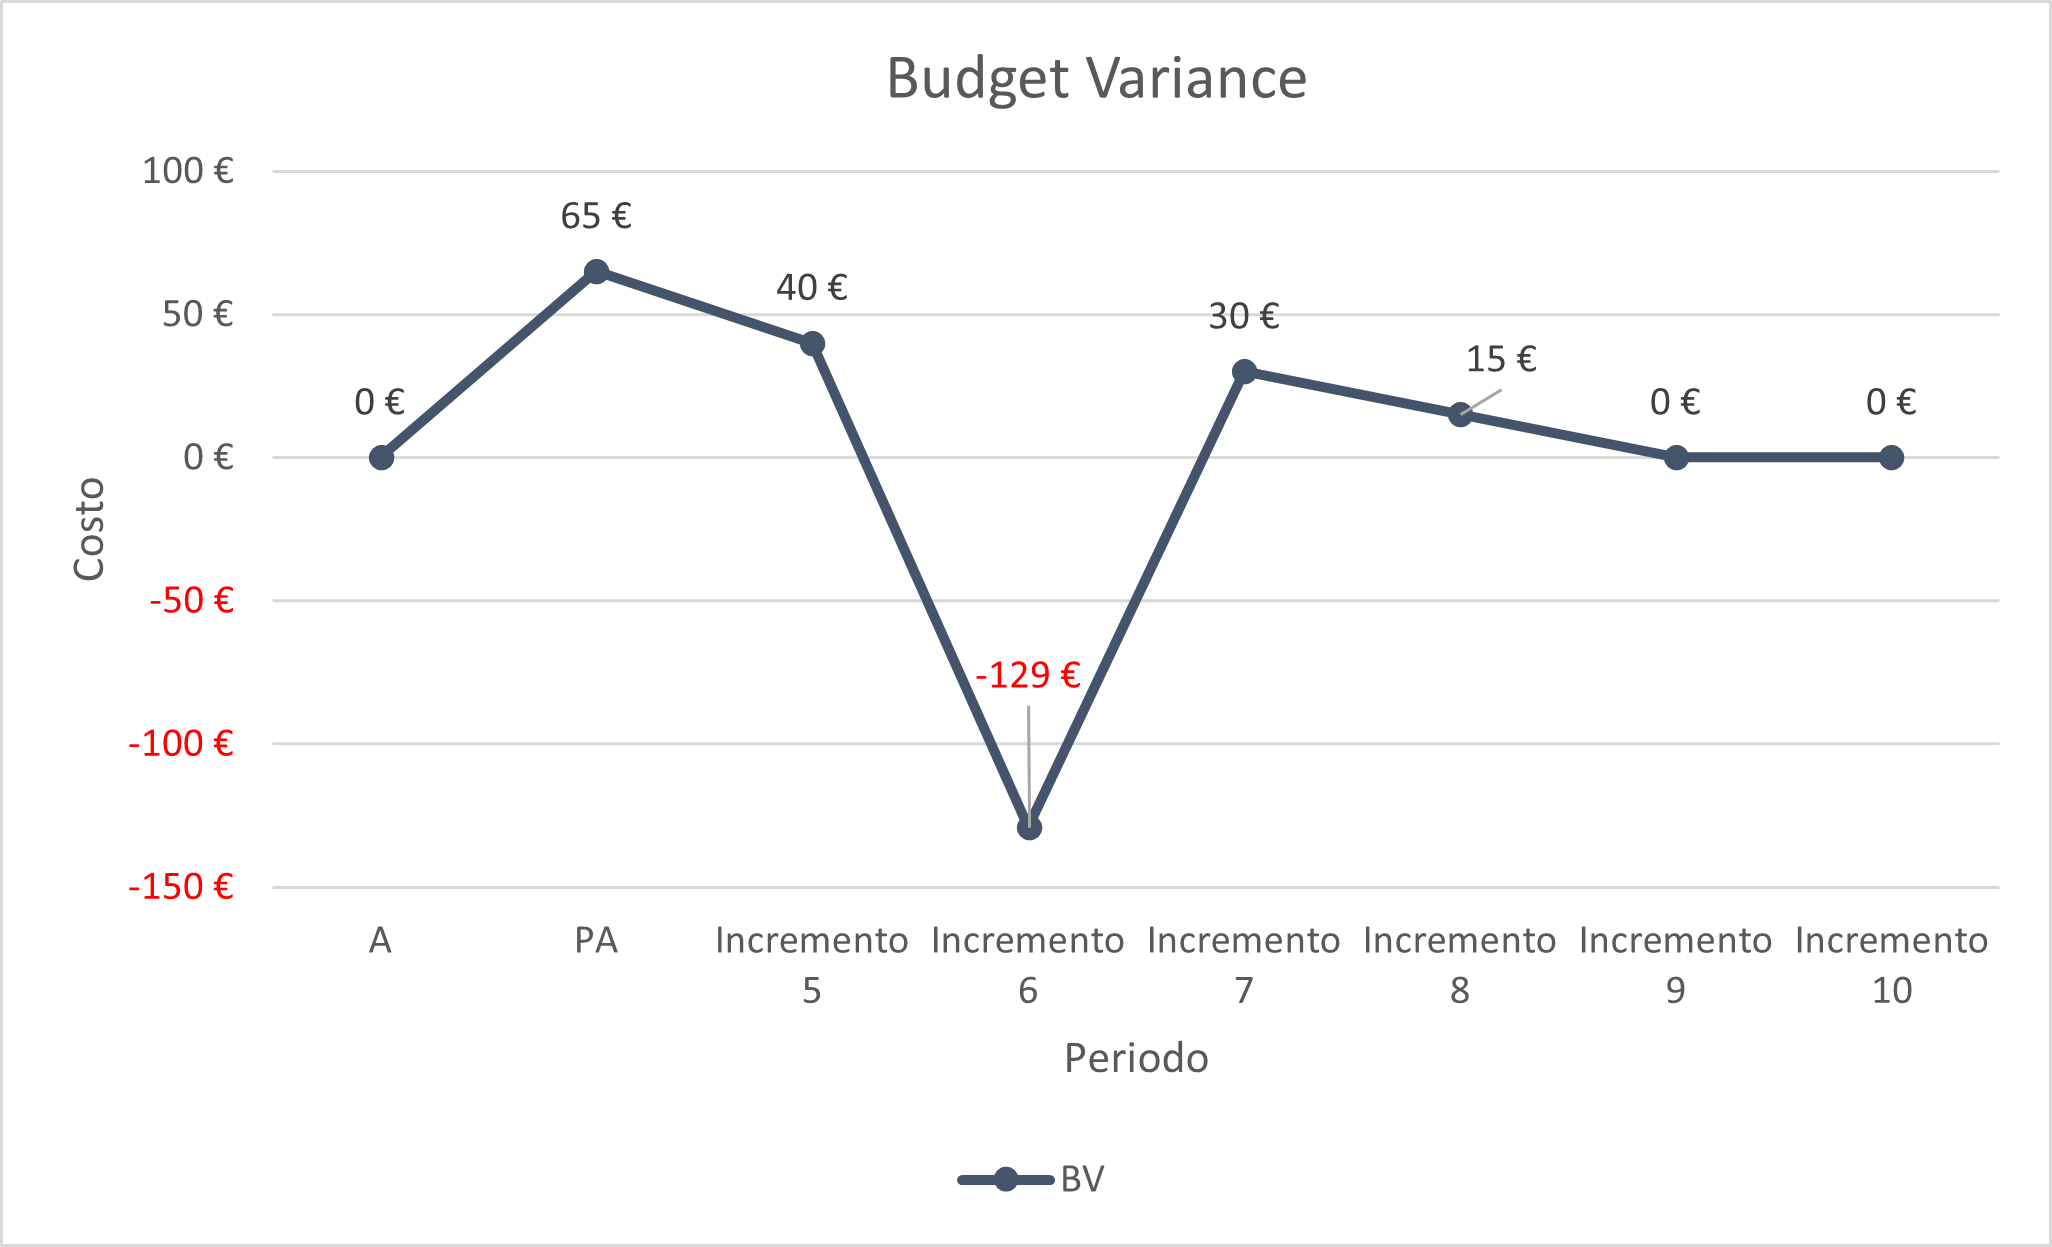
\includegraphics[scale=0.78]{res/ResocontoAttivitaDiVerifica/res/metriche/grafici/img/budgetVariance.png}\\
\caption{Andamento Budget Variance}
\end{figure}


\subsubsection{MPC11 - Percentuale di metriche soddisfatte}
Di seguito è riportato il grafico della percentuale di metriche soddisfatte, il cui valore è definito accettabile e ottimale come descritto nella sezione §2.3.2.1.\\

\begin{figure}[H]
\centering
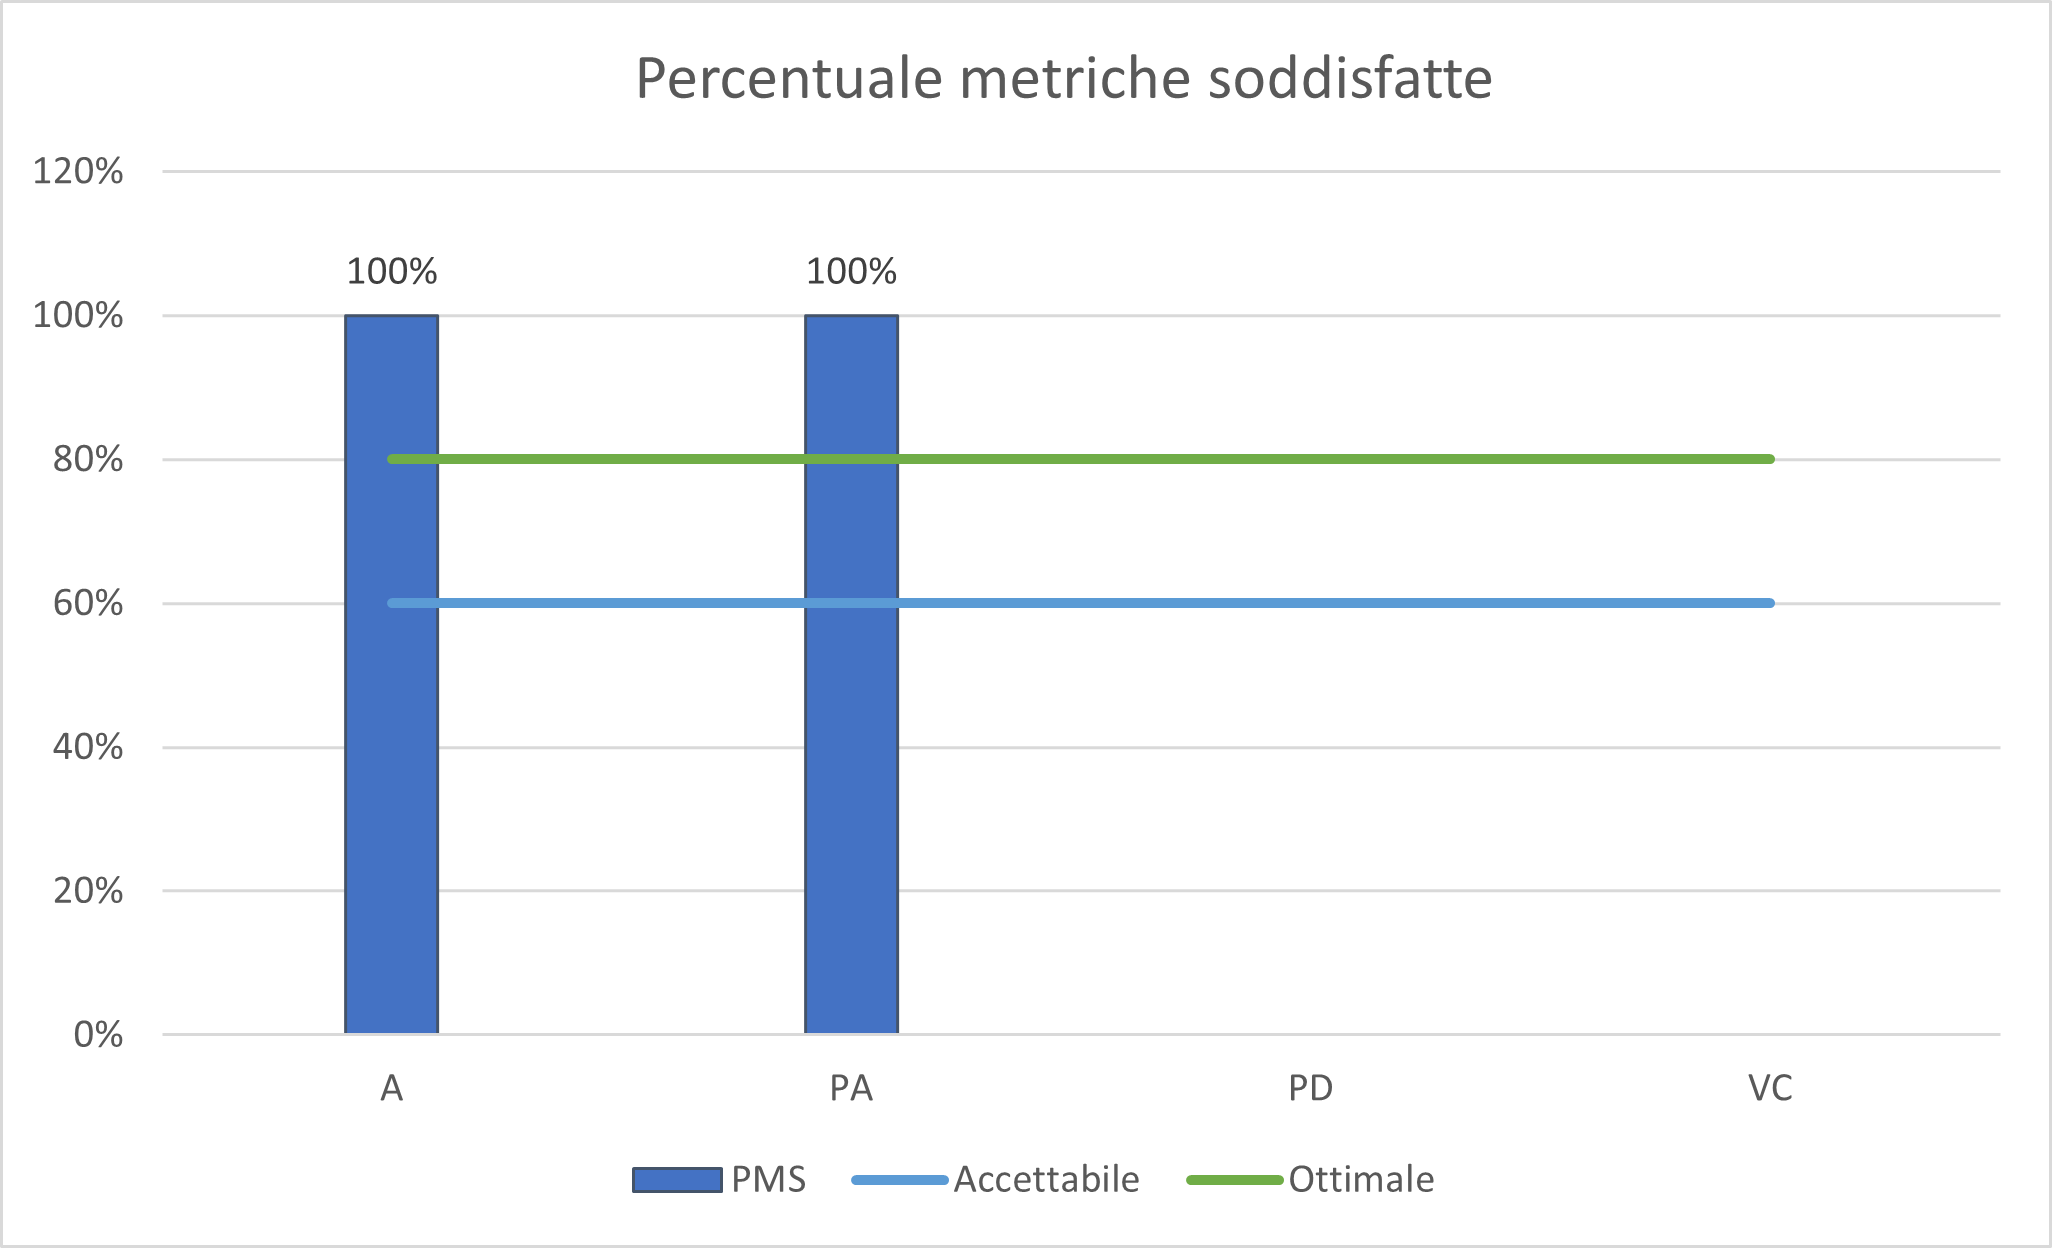
\includegraphics[scale=0.78]{res/ResocontoAttivitaDiVerifica/res/metriche/grafici/img/metricheSoddisfatte.png}\\
\caption{Andamento percentuale delle metriche soddisfatte}
\end{figure}

